\subsection{Justification}\label{subsec:justification}
The positive correlation between performance optimisation and energy optimisation is rather intuitive, as many
strategies for performance optimisation (such as reducing unnecessary execution) are congruent with energy optimisation.
This correlation appears to transcend programming languages themselves, with studies into energy usage of languages
coming up with similar ratios of energy against time for the same algorithms\cite{EnergyEfficiencyAcrossProgrammingLanguages}.

In comparison to performance profiling, energy profiling can be far more cumbersome to execute(SOURCES), this has lead to the
suggestion of using performance profiling as a proxy to loosely optimise energy cost\cite{PerformanceVEnergyMobile} with
papers suggesting that execution time can be used to directly infer energy cost\cite{ExecutionTimeVsEnergyCost}.

\subsection{Approach}\label{subsec:approach}
It is unlikely that a single ratio can model the relationship between performance and energy, this report will attempt
several methods at extrapolating contextual information of a script to predict its energy usage.
Certain programming concepts such as memory management and caching may require more advanced approaches to make accurate
predictions, such as multithreading, which has positive effects on performance at the cost of negative effects on energy
usage\cite{MultithreadingEnergy}.

To find the most accurate model, this report will attempt to use a variety of forecasting techniques to predict energy
readings from performance readings, then compared against actual energy readings to find the most accurate model.

\subsubsection{Experimental Space}
To prevent bias in specific operations, this paper will attempt to use a variety of scripts that perform different
purposes.
As a time constraint, the scripts should be simple to execute, and ideally should have very little ambiguity on their
intended execution - as an example, python libraries will not be considered, as they perform many functions, and it is
difficult to determine an execution path without a full understanding of the library.
Consequently, programs operate on a resource, or connect to the internet will also not be considered, to prevent
time wasted on debugging network issues or misunderstandings of the operable resource.

Constraining the experimental space like this introduces an obvious bias, this can be addressed in continuations of this
research by expanding the experimental space to include more complex scripts.

The most obvious approach is to start by running benchmarks, as they are often designed to test the limits of a system
and are likely to explore a wide range of operations to draw conclusions.
For this report we will use the scripts defined in the Debian computer languages benchmark game\cite{BenchmarkGame}.
Relying on benchmarks has two major drawbacks: the first is that benchmarks necessarily are not a good representation
of a typical use case of a system, rather a way to expose the flaws of the tested system; the second issue is that
benchmarks must be designed to be comparable across the tested systems - in our case this means that all the algorithms
we have taken from the benchmark games were chosen for their broad applicability and may not cover a sufficient amount
of Python constructs to be useful for our purposes.
Nevertheless, the benchmarks will provide a good starting point for our research.
In a parallel approach, we can find example code to benchmark specific sectors by searching for research papers
comparing technologies in that sector, this provides a more focused approach to targeting specific concepts in Python,
as sufficiently well presented papers will provide control groups to eliminate technology bias.
For this report we have identified [TODO FILL IN]

The next natural avenue to search is example code for certain functionalities, unfortunately this is also very use-case
specific.
For this report we will experiment with taking solutions from Project Euler\cite{ProjectEuler}, a website that provides
mathematical puzzles that can be solved using algorithms - with almost 1000 problems, there should be significant
coverage of various Python constructs used to solve them.

Each chosen set of algorithms has a clear bias towards their intended use, the intent of this section is to provide an
experimental space that is not constrained by a single problem space.
Unfortunately the algorithms listed would take a significant amount of time to test, so we must further narrow the space
by choosing subsets of each set of algorithms that best represent their respective biases.
Our first attempt at making this choice is to use the disassembler module to ensure that a large amount of opcodes are
covered in the executions.
Unfortunately any kind of curation requires a manual review process, which is constrained by time, this introduces the
possibility of certain operations being underrepresented in the results.

\subsubsection{Data Collection}\label{subsubsec:intro-data-collection}
Data collection will be done using the RAPL interface, which is widely accepted as a sufficiently reliable method of
measuring energy[SOURCES].

The RAPL interface has multiple points of access, which on Linux all depend on the \textit{powercap}
framework\cite{LinuxPowerCap} this section will explore the best approaches to collecting data from RAPL to get the best
test results.
For the purposes of our experiments we will retrieve the energy values in micro-Joules directly from the framework (this
can be done simply by reading the files exposed in the powercap interface).
Our method for retrieving this data is to manually find where each RAPL domain is stored, and retrieving the number that
is stored there - later we can compare these numbers to retrieve a delta of energy usage.
To have a better idea of the energy usage throughout a script's execution, we will retrieve the energy usage at regular
intervals throughout the script's execution, this will also help identify any anomalous behaviour in the energy usage.
The disadvantage of this is similar to the disadvantage of physical energy meters, as there is no way to guarantee that
the beginning of the script is synced with the first energy reading, multiple experiments can mitigate this issue.

The first and easiest way to measure the energy usage of a script is to measure the energy before and after, this
functionality is provided quite simply via the perf tool.
To understand the affect of individual constructs on execution time, there is a need for a more granular measurement of
energy, this can be done one of two ways - either by injecting energy measurements into the scripts themselves, or
by having a separate process measuring the energy level at specified intervals.
The first approach has the advantage of being able to measure the energy usage of the components themselves, while the
second approach is much less invasive and can be applied broadly.
Due to the structured nature of RAPL interface writes, an outside polling approach seems to be more advantageous, as
more granular measurements will not necessarily provide additional data - although this does introduce the possibility
of synchronisation issues between the script and the polling process.

Our first attempt at a polling process for energy usage is with the use of a cron job that runs every second, the job
is simply a bash script that saves data points to a logfile that can then be plotted.
In the interest of a full picture, we also retrieve the temperature statistics of the machine, as it may help to
explain anomalous behaviour in the results we find.
Unfortunately cron does not expose the ability to run a script at a higher frequency than once a minute, so we must
implement a script that executes the polling process in a loop at 1 second intervals.
This has two disadvantages: firstly, if there is any interruption of the script, the polling process will be offset (
if the script is delayed by a second, then there will be a 2-second gap between measurements, and consequently a
duplicate value at the start of the next minute); additionally, as the script executes in non-zero time, every execution
will delay the next poll, this means that the interval does not remain consistent even with perfect execution.
Finally, in the event that the results of this report are to be reproduced, it should be noted that the cron service is
not a guaranteed part of all Linux systems, and may have to be manually installed.

\begin{figure}[H]
    \centering
    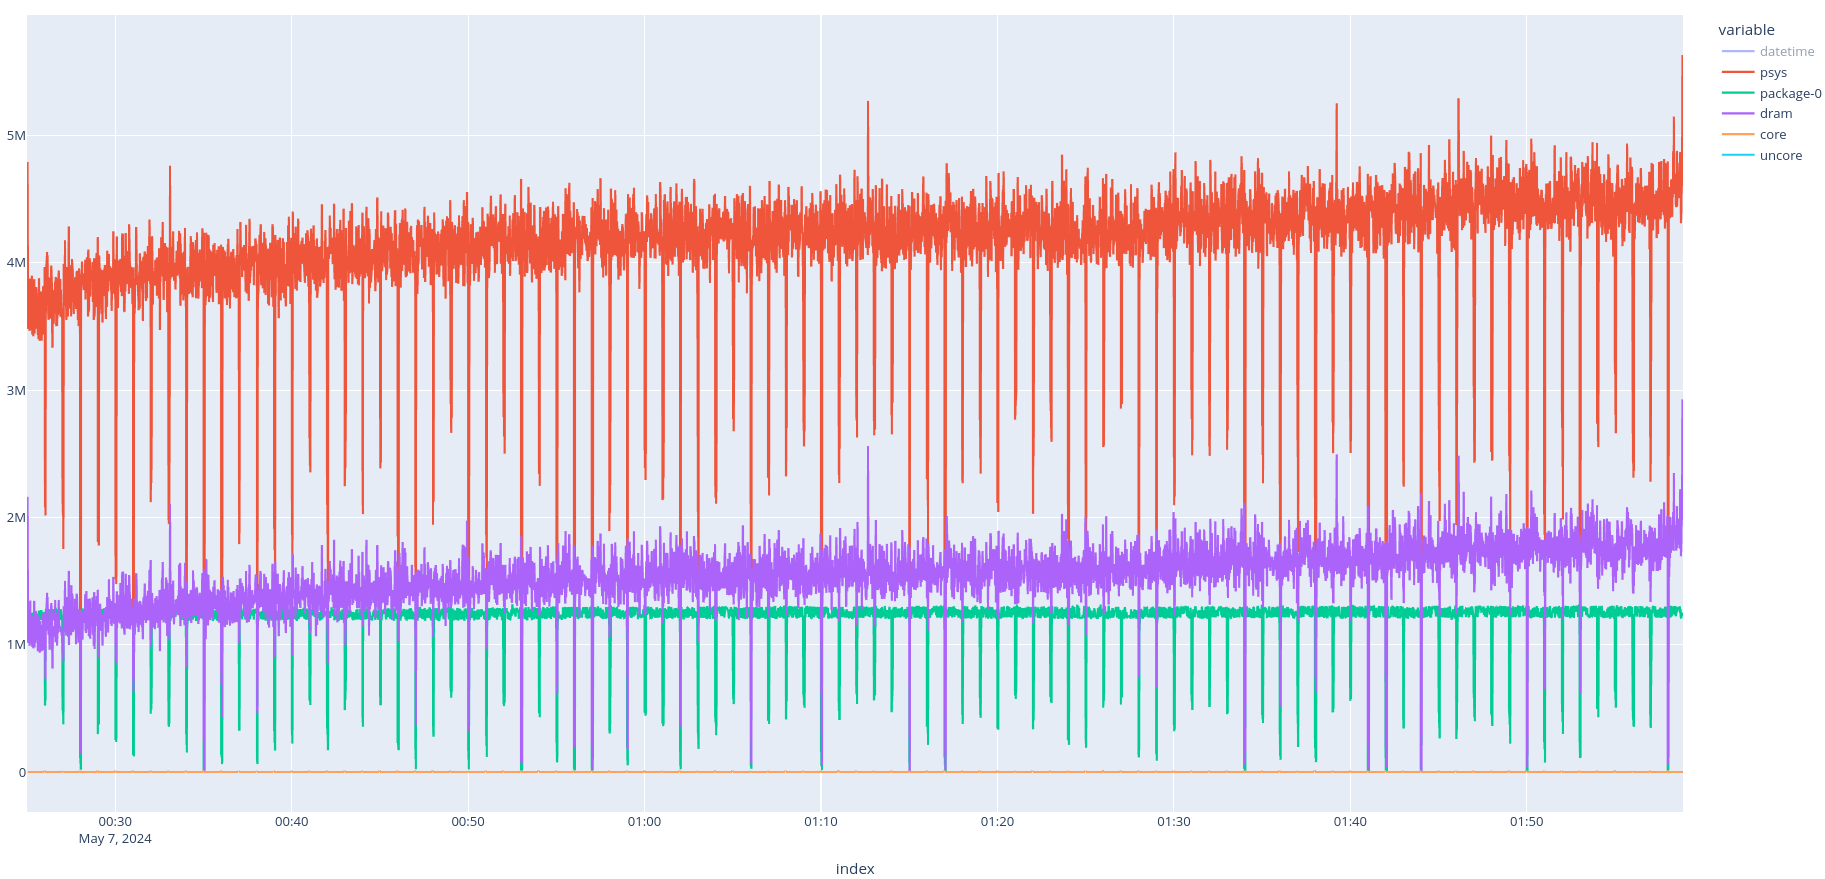
\includegraphics[width=15cm]{figures/introduction/crontab_energy_polling}
    \caption{Using crontab to poll for energy usage every second, the inconsistency of intervals can be seen to cause
    spikes in the data that would have to be normalised for a more accurate representation of the data.}
    \label{fig:crontab_energy_polling}
\end{figure}

The next logical step is to attempt to take advantage of the systemd service manager, which allows creation of custom
daemon services, this includes a timer functionality that allows us to run a polling script every second.
As we can see in~\ref{fig:systemd_energy_polling}, the systemd service provides a more consistent interval between
polls, which reduces variance.

\begin{figure}[H]
    \centering
    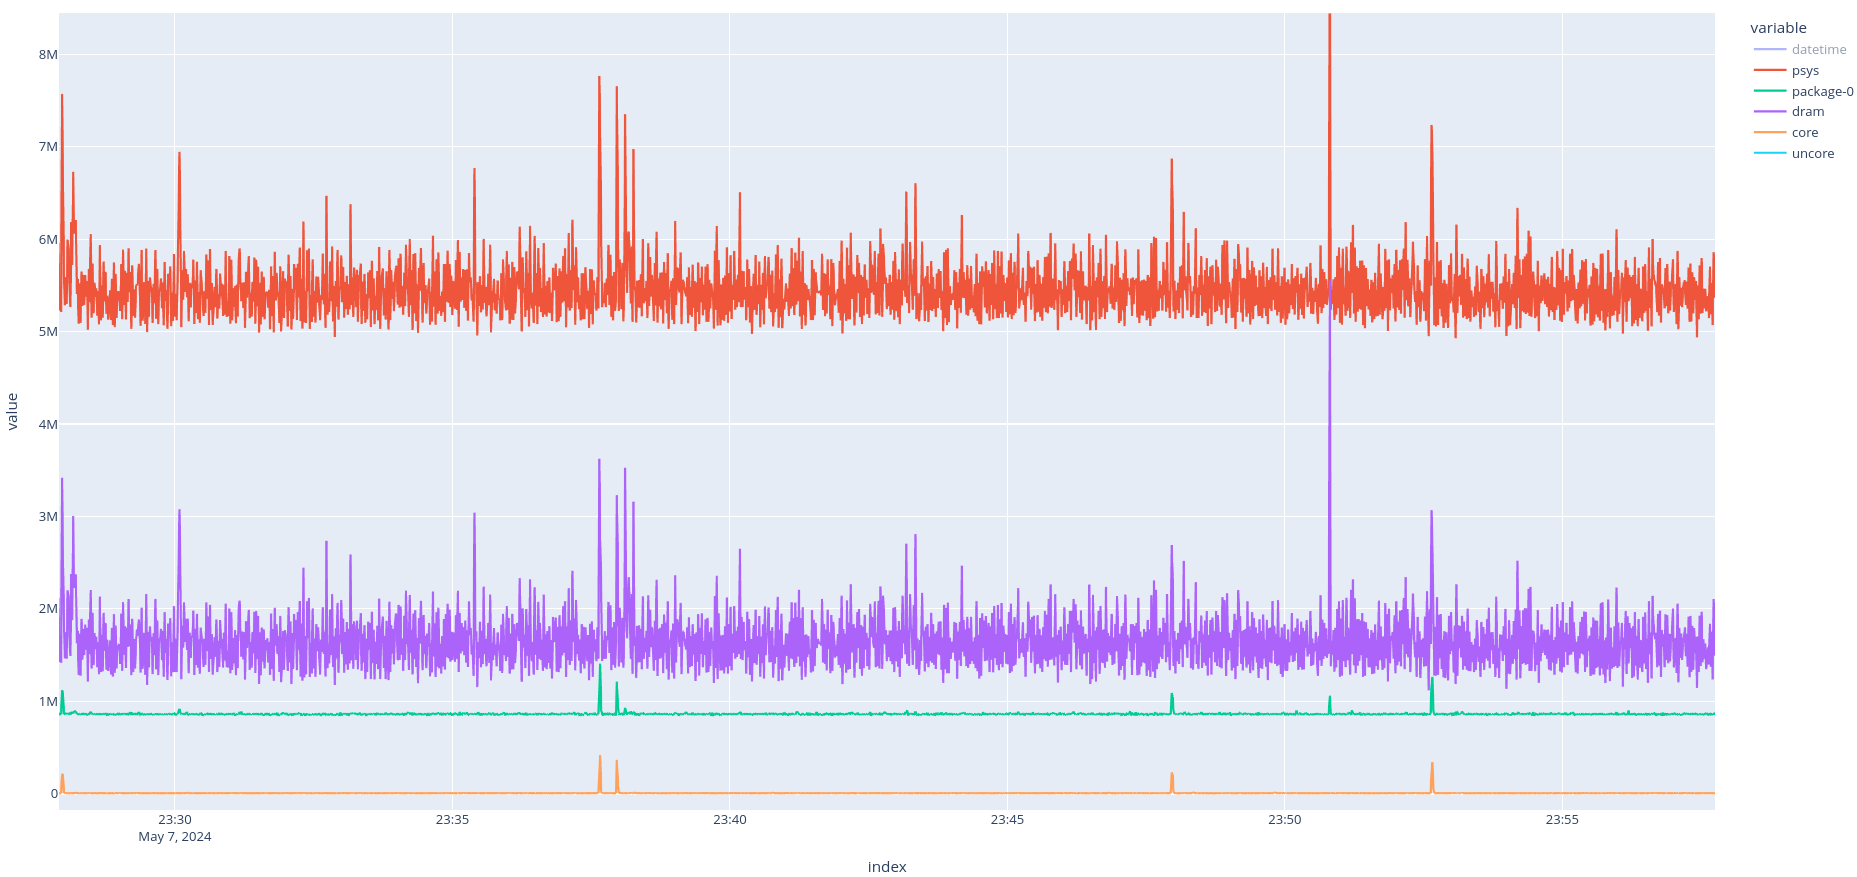
\includegraphics[width=15cm]{figures/introduction/systemd_energy_polling}
    \caption{Using systemd to poll for energy usage every second, the consistency of intervals can be seen to provide a
    more consistent data set, however there is still clear visible variation in the data that may pollute results}
    \label{fig:systemd_energy_polling}
\end{figure}

\begin{lstlisting}[caption={power and temperature logging script},captionpos=b,label={lst:powerlog-script}]
ENERGYOUT=###############
TEMPOUT=#################
ENERGY_FILE=$(cat ###############)

time=$(date +"%y-%m-%d %T")
energy=$(cat $ENERGY_FILE | sed -z 's/\n/,/g')
temp=$(sensors | awk -F '°' '/^Core/{gsub("[[:space:]]+",""); printf "%s,", $1}')

echo "RUNNING POWERLOG"
printf "$time,$energy\n" >> $ENERGYOUT
printf "$time,$temp\n" >> $TEMPOUT
\end{lstlisting}
\begin{lstlisting}[caption={systemd service},captionpos=b,label={lst:systemd-energy-polling}]
[Unit]
Description=Run profiler every second
StartLimitIntervalSec=60
StartLimitBurst=61

[Service]
ExecStart=/usr/bin/bash #########/powerlog.sh
User=#######

[Install]
WantedBy=multi-user.target
\end{lstlisting}
\begin{lstlisting}[caption={systemd timer},captionpos=b,label={lst:systemd-energy-timer}]
[Timer]
OnUnitActiveSec=1s
AccuracySec=1us
Unit=profiler.service
\end{lstlisting}
